%%&program=xelatex
%&encoding=UTF-8 Unicode
% SVN keywords
% $Author$
% $Date$
% $Revision$
% $URL$
\documentclass[a4paper,12pt]{article}      % Comments after  % are ignored
%\usepackage{hyperref}                 % For creating hyperlinks in cross references
%
\usepackage{ifxetex}% for XELATEX, or PDFlatex
\usepackage{ifplatform} 
%
\ifxetex
	\usepackage{polyglossia} \setmainlanguage{portuges}
	\usepackage{fontspec}
	\ifwindows
		\setmainfont[Ligatures=TeX]{Garamond}
		\setsansfont[Ligatures=TeX]{Gill Sans MT}
		\setmonofont[Scale=MatchLowercase]{Courier}
	\fi
	\iflinux
		\setmainfont[Ligatures=TeX]{Linux Libertine O}
		\setsansfont[Ligatures=TeX,Scale=MatchLowercase]{Linux Biolinum}
		\setmonofont[Scale=MatchLowercase]{Courier}
	\fi
	\ifmacosx
	% add settings
	% Use xelatex -no-shell ...
	\fi
	\usepackage{xcolor,graphicx} 
\else
	\usepackage[portuguese]{babel}
	%\usepackage[latin1]{inputenc}
	\usepackage[utf8]{inputenc}
	\usepackage[T1]{fontenc}
	\usepackage{graphics}                 % Packages to allow inclusion of graphics
	\usepackage{color}                    % For creating coloured text and background
\fi

\usepackage{enumitem}
\setlist{nolistsep}
\usepackage{amsmath,amssymb,amsfonts} % Typical maths resource packages

\oddsidemargin 0cm
\evensidemargin 0cm

\pagestyle{myheadings}         % Option to put page headers
                               % Needed \documentclass[a4paper,twoside]{article}
\markboth{{\small \it  Laboratório de Física Experimental Básica}}
{{\small\it MEFT - LFEB 1º Sem. 2014/2015} }

\addtolength{\hoffset}{-0.5cm}
\addtolength{\textwidth}{2.5cm}
\addtolength{\topmargin}{-1.5cm}
\addtolength{\textheight}{3cm}

%\textwidth 15.5cm
%\topmargin -1.5cm
\setlength{\parindent}{0pt}
\setlength{\parskip}{1ex  plus  0.5ex  minus  0.2ex}
%\parindent 0.5cm
%\textheight 25cm
%\parskip 1mm


% Math macros
\newcommand{\ud}{\,\mathrm{d}} 
\newcommand{\HRule}{\rule{\linewidth}{0.5mm}}

\author{Prof. Bernardo B. Carvalho} 

%%%%, Bernardo Brotas Carvalho\\bernardo@ipfn.ist.utl.pt} 
\date{ Outubro 2012} 

\begin{document} 

	
\includegraphics[width=0.2\textwidth]{../logo-ist}%\\[1cm]  %%  Logo_IST_color

	\HRule \\[0.5cm]
	{ \huge \sf  \textsc{Velocidade da Luz} }\\[0.4cm] % \bfseries 
%	{ \large \bfseries Determinação Experimental da Carga $q$ do Eletrão }\\
%	{ \large \bfseries Procedimento Experimental}\\
	\HRule \\%[0.5cm]


\section{\sf Introdução}
Em muitas das experiências descritas na literatura para
determinacão da velocidade da luz foram utilizados feixes luminosos
pulsados (ou modulados), que percorrem determinados trajetos de maior ou menor
comprimento (Fig. \ref{fig:Fizeau}). 
No presente trabalho utiliza-se como fonte luminosa um díodo que
emite radiação eletromagnética visível com um comprimento de onda na
zona do vermelho. A tensão aplicada ao díodo emissor é alternada
sinusoidal de frequência $f_{mod}=50\,MHz$ e  assim a intensidade sinal luminoso
 emitido é \emph{Modulado em Amplitute} (AM), naquela frequência. 

\begin{equation*}
	\label{eq:f_am}
		s_{diodo}(t) = A(t) \cdot \sin ( 2\pi \cdot f_{luz} \, t) = \underbrace{A_0 \sin ( 2\pi \cdot 50\times 10^6 \, t)}_\text{Amplitude Modulada} \cdot \sin ( 2\pi \cdot f_{luz} \, t)
\end{equation*}

\begin{figure}
	[ht!b]  \centering 
	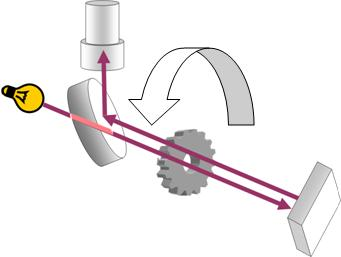
\includegraphics[width=0.5\textwidth]{Fizeau}
	\caption{Esquema do aparelho para determinar a Velocidade da Luz utilizado por Fizeau em 1849. \label{fig:Fizeau}} 
\end{figure}

%\section{\sf Introdução}

\section{\sf Base do Método}
No presente trabalho o feixe luminoso proveniente do díodo emissor
é forçado a percorrer um determinado trajeto sendo em seguida detetado
por um foto-díodo receptor (Fig. \ref{fig:Montagem}). O sistema de espelhos $E_1\,E_1$, pode deslocar-se ao longo de uma calha graduada,
sendo assim possível variar o comprimento do trajeto do raio luminoso. Os
sinais de amplitude impostos ao emissor e captados no receptor são aplicados\footnote{Depois de uma deteção \emph{heterodínica}, em que a frequência modulada é desviada \\ 
$f_{bat}=50\, MHz -50.050\, MHz = 50\,kHz$. Esta operação permite a utilização de um osciloscópio de banda de frequências mais reduzida.} 
aos canais de um osciloscópio funcionando em modo “XY”.

O sinal visualizado no osciloscópio é uma figura de Lissajous e como em ambos os sinais vertical e horizontal a frequência é a 
mesma\footnote{Na realidade são sinais \emph{coerentes}, pois provêm da mesma fonte}, é uma elipse com a equação geral:
\begin{equation}
	\label{eq:elipse}
	\sin^2 \delta = \frac{A_x^2}{A_{x0}^2} + \frac{A_y^2}{A_{y0}^2} - \frac{2 A_y\,A_x}{A_{y0}\,A_{x0}} \cos  \delta
\end{equation}

\begin{figure}
	[htb]  \centering 
	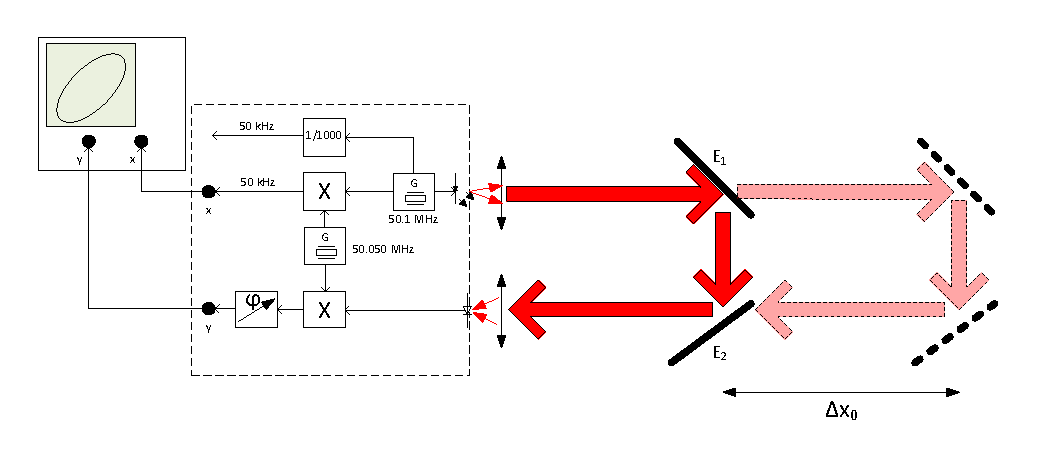
\includegraphics[width=0.8\textwidth]{Vel_esquema}
	\caption{Montagem no Laboratório para determinar a Velocidade da Luz. \label{fig:Montagem}} 
\end{figure}

Sendo $A_x(t)$ o sinal de intensidade captado no emissor,  $A_{x0}$ a sua amplitude máxima,  $A_y(t)$ o sinal
proveniente do recetor, $A_{y0}$ a sua amplitude máxima e $\delta$ a desfasagem entre os dois
sinais. O ângulo $\delta$ irá variar com a trajecto do raio luminoso.  A elipse pode degenerar em retas quando os dois sinais estiverem
em fase, $\delta = 2n\,\pi$ (nos quadrantes ímpares)  ou em oposição de fase, $\delta = (2n+1)\,\pi$ (nos quadrantes pares). 

\subsection{\sf Velocidade da Luz no ar}
Neste trabalho a
velocidade da luz é calculada a partir da determinação do comprimento do
caminho suplementar, ($2\,\Delta\,z$), que a luz tem de percorrer para que se passe de uma
situação em que os sinais estão em oposição de fase à situação contígua de
fase. Assim a luz percorre esse comprimento suplementar num intervalo de
tempo, ($\Delta t$) ,  que é igual a metade do periodo ($T/2$) do sinal modulante ($T=1/50\,MHz= 20\,ns$). 

\begin{figure}
	[htb]  \centering 
	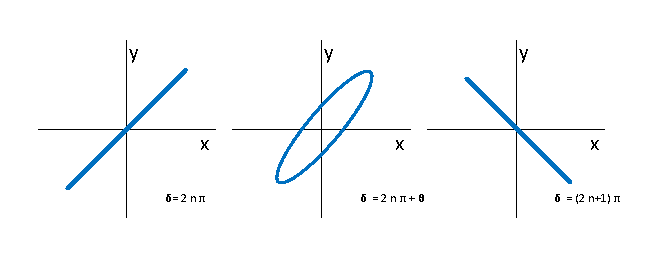
\includegraphics[width=0.8\textwidth]{osci_fase}
	\caption{Figuras de Lissajous observadas no osciloscópio. \label{fig:fase}} 
\end{figure}

No ar teremos:
\begin{equation}
	\label{eq:vc}
	c_{ar} = \frac{2\,\Delta z_0}{T/2} 
\end{equation}

\subsection{\sf Velocidade da Luz em meios sólidos e líquidos}
 O índice de refração de a um meio material $1$ em relação a um meio material $0$
 para um dado comprimento de onda pode ser definido \footnote{Esta definição só é válida se as condutividades dos meios $0$ e $1$ forem nulas, ou seja nos \emph{dielétricos} perfeitos.}
 como a relação entre as velocidades de propagação da luz nos meios $0$ e $1$:

 \begin{equation}
	\label{eq:index}
	n_1 \equiv \frac{c_0}{c_1}  = \frac{\frac{1}{\sqrt{\varepsilon_0 \, \mu_0}} }{\frac{1}{\sqrt{\varepsilon_1 \, \mu_1}} } =
		\sqrt{\frac{\varepsilon_1 \, \mu_1}{\varepsilon_0 \, \mu_0}} = \sqrt{\varepsilon_r \, \mu_r}
\end{equation}

Nesta expressão $\varepsilon_0$, $\varepsilon_1$ e $\varepsilon_r$   e  $\mu_0$, $\mu_1$, e $\mu_r$ são as constantes dielétricas  as permeabilidades magnéticas respetivamente do meios $0$ e $1$ e a relativa $(\varepsilon_1= \varepsilon_r\, \varepsilon_0)$.

\begin{figure}[h!tb]  
	\centering 
	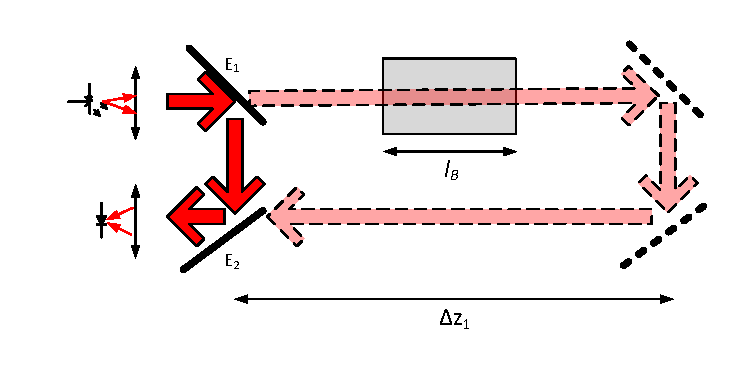
\includegraphics[width=0.8\textwidth]{Vel_esquema_bloco}
	\caption{Montagem para determinar índices de refração em sólidos e líquidos. \label{fig:Montagem_bloco}} 
\end{figure}

Se no percurso do feixe luminoso interpormos um bloco de material sólido ou líquido transparente 
 de comprimento $l_B$ (Figura \ref{fig:Montagem_bloco}) então a expressão  (\ref{eq:vc}) pode ser generalizada em:

\begin{equation}
	\label{eq:vc_bloco}
	{T/2}  = \frac{2\,\Delta z_1 - l_B}{c_{ar}}  +  \frac{l_B}{c_{B}}
\end{equation}
De onde se pode pode extrair a velocidade $c_{B}$. 

Pode obter-se directamente o indíce de refração $n_{B}$, a partir de (\ref{eq:vc}) e (\ref{eq:index}).

\begin{align}
	\label{eq:n_bloco}
	{T/2}  = \frac{2\,\Delta z_0}{c_{ar}}  &=  \frac{2\,\Delta z_1 }{c_{ar}} -   \frac{l_B}{c_{ar}}  +  \frac{l_B}{c_{B}} \nonumber \\ 
	\frac{2\,(\Delta z_0- \Delta z_1 )}{c_{ar}}  &= -   \frac{l_B}{c_{ar}}  +  \frac{l_B}{c_{B}} \nonumber \\
	\frac{2\,(\Delta z_0- \Delta z_1 )}{l_B} &= -1 +  \frac{c_{ar}}{c_{B}} \nonumber \\
	n_{B} &= 1 +  \frac{2\,(\Delta z_0- \Delta z_1 )}{l_B} 
\end{align}

 Neste trabalho será  determınada os índices de refração, e a velocidade da
luz, em  mais dois meios materiais, a resina acrílica e a água. 
 

\subsubsection{\sf Questões a responder ANTES da sessão de Laboratório:}
\begin{enumerate}
\item A luz emitida pelo díodo tem um comprimento de onda de $\lambda \approx 600 \, nm$. Calcule $f_{luz}$ e compare com a frequência da amplitude.
\item Explique porque razão nesta experiência a luz utilizada  tem de ter a intensidade variável.
%, tal como na experiência da Velocidade do Som.
\item Uma outra montagem desenvolvida no IST utiliza um díodo laser de longo alcance. No entanto apenas se consegue modular a $f_{mod}=1\, MHz$. Calcule a distância
dos espelhos necessária para se obter o efeito de oposição de fase entre a amplitude do sinal emitido e o recebido.
\end{enumerate}

\newpage
\section{\sf Protocolo Experimental}
\subsection{\sf Material utilizado}

\begin{enumerate}
\setlength{\itemsep}{0mm}
\item Unidade de emissão de luz (díodo emissor) e de recepção (díodo receptor)
(amplitude modulada por um sinal de frequência $50\,MHz$).
\item Duas lentes plano-cilíndricas.
\item Conjunto de dois espelhos planos para inversão do sentido de propagação da luz.
\item Calha graduada.  
\item Bloco de vidro acrílico transparente.
\item Dois tubos com cerca de 1 metro de comprimento para conter água ou ar. 
\item Osciloscópio de dois canais a funcionar em modo “XY”.
\end{enumerate}

\subsection{\sf Procedimento Experimental}
\subsubsection{\sf Regulação da montagem}
 
Comece por verificar se a montagem ótica está devidamente alinhada. Teste a evolução da forma da mancha 
luminosa ao longo do percurso óptico usando um alvo difusor (por exemplo, papel vegetal). 
Verifique que a mancha está centrada com  orifício que permite iluminar o 
díodo receptor. Coloque a lente no lado do díodo receptor.
Ajuste os parafusos dos espelhos de forma a maximizar a amplitude do sinal 
recebido.
Coloque os espelhos na posição zero da escala e, rodando o botão que modifica 
continuamente a diferença de fase entre os dois sinais, obtenha uma reta dos quadrantes ímpares. 

\subsubsection{\sf Velocidade de propagação da luz no ar}
Desloque os espelhos sobre a calha e observe a modificação da figura no ecrã do 
osciloscópio, em particular, nas posições que correspondem aos sinais recebidos estarem 
desfasados de $\pi/2$ (quadratura) e em oposição de fase. Para esta última situação registe a 
posição dos espelhos e o intervalo, $e_z$,  para o qual os sinais parecem estar ainda em 
oposição de fase. Repita a medida pelo menos duas vezes (cada observador). 
Calcule a velocidade de propagação da luz no ar, a sua incerteza e o desvios à exatidão\footnote{O valor $c_{ar}$ é muito próximo de $c_{vacuo} = 299 792 458\,m/s$, que é uma constante exacta do Sistema Internacional de Medidas. O índice de refração do ar para a luz visível é $n_{ar}=1.000293$}. 

\subsubsection{\sf Velocidade de propagação da luz no vidro acrílico}
Verifique de novo se no zero da escala de posição os sinais estão em fase. Coloque o bloco de vidro 
acrílico no feixe incidente de modo que entre perpendicularmente às faces e faça o percurso 
mais longo no vidro acrílico. Meça a posição e a incerteza correspondente dos espelhos para que 
que os dois sinais detetados estejam em oposição em fase. Repita a medida pelo menos 
duas vezes (cada observador).
Calcule o índice de refração obtido para o vidro acrílico, $n_{vidro}$, pela expressão (\ref{eq:n_bloco}),  e a sua incerteza. Calcule o valor da velocidade.

\subsubsection{\sf Velocidade de propagação da luz na água}
Verifique de novo que no zero da escala do espaço os sinais estão em fase. Coloque o tubo vazio de 
água nos suportes de modo que o feixe incidente entre perpendicularmente às faces.
Registe a posição dos espelhos que produz um sinal em oposição de fase com o incidente. 
Repita estas medidas para o tubo cheio de água. 
Calcule o valor da índice de refração obtida para a água $n_{agua}$, a sua incerteza e os desvio à exatidão\footnote{O valor tabelado é $n_{agua}=1.3330$}. 
Comente a precisão do valor da velocidade de propagação da luz obtida nos 
diferentes meios.
\end{document} 